\documentclass[11pt,a4paper]{article}
\usepackage{amsfonts}
\usepackage{amsmath}
\usepackage{amsthm}
\usepackage[utf8]{inputenc}
\usepackage{hyperref}
\usepackage{graphicx}
\usepackage{pgfplots}
\usepackage{pgfplotstable}

\usepackage{minted}
\newminted{py}{%
%		linenos,
		fontsize=\footnotesize,
		tabsize=2,
		mathescape,
}
\newminted{text}{%
%		linenos,
		fontsize=\footnotesize,
		tabsize=2,
		mathescape,
}

\usepackage{xcolor}

% \toprule, \midrule and \bottomrule in tables
\usepackage{booktabs}

\newcommand{\norm}[1]{\left\lVert#1\right\rVert}

\newcommand*\mat[1]{ \begin{pmatrix} #1 \end{pmatrix}}
\newcommand*\arr[1]{ \begin{bmatrix} #1 \end{bmatrix}}
\newcommand*\V[1]{ \boldsymbol{#1}}

\newcommand*\D{\textcolor{violet}{D}}
\newcommand*\T{\textcolor{blue}{T}}

\title{Approximated PCA}
\author{Rodrigo Arias Mallo}

\begin{document}
\maketitle

\section{Introduction}

The PCA method transforms a set of observations of possibly correlated variables 
into a set of values of linearly uncorrelated variables called principal 
components using an orthogonal transformation (rotations and reflections).

The transformation, projects the data in a new subspace, in which each new 
variable it's now uncorrelated. That means that the covariance of each pair of 
new variables is zero.
%
To compute the transformation, different approaches can be taken. In a first 
attempt, the covariance matrix will be used.
%
Let $x_{ij}$ be the observation $j$ of the variable $i$. Let $n$ be the number 
of variables and $m$ the number of observations.
%
Each element $s_{ij}$ in the covariance matrix $S$ is computed by
%
$$ s_{ij} = \frac{\sum x_{ik} x_{jk} - \sum x_{ij} x_{jk}}{n (n-1)} $$
%
Once the covariance matrix $S$ in computed, it can be used to find his 
eigenvalues and eigenvectors. One method to compute those values, is a 
combination of a Householder transformation, followed by the QR transformation.  
The first will transform $S$ in a product of two matrix $Q$ and $R$.
%
	$$ S = QR $$
%
Such that $R$ contains 3 diagonals (tridiagonal) with elements and zeros in the 
rest. The QR transformation then takes this two matrices, and computes 
iteratively a new diagonal matrix $A^{(i+1)} = R^{(i)} Q^{(i)}$. Finally, the 
eigenvalues are in the diagonal of $A$ and the eigenvectors are computed from 
these.

\section{Householder tridiagonalization}

The Householder tridiagonalization it's a process where a matrix $A$ is 
transformed by multiplying with an orthogonal matrix $P^{(k)}$:
%
$P^{(k)} = I - 2ww^T$
%
Such matrix $P^{(k)}$ has been prepared, so that $P^{(k)}A$ is a new matrix, 
with zeros below the $k+1$ element in the $k$ column. This new matrix, has the 
same eigenvalues as the provious $A$. The step is repeated until the final 
matrix has only elements in the diagonal, and the two sub-diagonals. The process 
is similar to a Gaussian elimination.

\section{Eigenvalue sensitivity}

% Extracted from Golub, Van Loan - Matrix multiplications.

Corolary 8.1.6: If $A$ and $A+E$ are \textit{n-by-n} symmetric matrices, then
%
$$ |\lambda_k(A+E) - \lambda_k(A)| \le \norm{E}_2 $$
%
for $k = 1:n$.

Then, the difference between the eigenvalue of a noisy matrix, and the original, 
can be bounded by the 2-norm of $E$, also the maximum eigenvalue of $E$.

\section{First approach}

The first experiment to be carried out consists in determining which parts of 
the algorithm can be suitable for approximate computing. The main steps of PCA 
can be summarized as follow:
%
\begin{enumerate}
\item Take a dataset $X$ of $n$ variables.
\item Scale and center the variables.
\item From $X$ compute the $n\times n$ covariance matrix $S$.
\item \textbf{Compute the eigenvalues and eigenvectors of $S$.}
\item \textit{Optional: Ignore some eigenvectors.}
\item Generate a new basis from the selected eigenvectors.
\item Project $X$ into the new basis.
\end{enumerate}
%
Computing the eigenvectors is the principal step of PCA.

\subsection{Computing eigenvalues and eigenvectors}

\begin{enumerate}
\item Take the $n\times n$ target matrix $A = S$.
\item Compute a tridiagonal matrix $T$: $A = P T P^T$.
\item From $T$ compute a diagonal matrix $D$: $T = Q D Q^T$.
\item The eigenvalues of $A$ are in the diagonal of $D$.
\item Compute the eigenvectors from $D$.
\end{enumerate}
%
Computing a tridiagonal matrix is called \textbf{tridiagonalization}. For the 
diagonal, \textbf{diagonalization}. Several algorithms exists for both steps.

\subsection{Tridiagonalization algorithms}

These algorithms transform a \textbf{symmetric} matrix $A$ into a new pair of 
matrices $P$ and $T$ such that $P$ is orthogonal, $T$ is tridiagonal, and $A = 
P T P^T$
%
$$
	\mat{
		a_{11} & a_{12} & a_{13} & a_{14} \\
		a_{21} & a_{22} & a_{23} & a_{24} \\
		a_{31} & a_{32} & a_{33} & a_{34} \\
		a_{41} & a_{42} & a_{43} & a_{44} \\
	} =
	P
	\mat{
		t_{11} & t_{12} &        &        \\
		t_{21} & t_{22} & t_{23} &        \\
		       & t_{32} & t_{33} & t_{34} \\
		       &        & t_{43} & t_{44} \\
	}
	P^T
$$
%
Some algorithms can be used for this factorization:
%
\begin{center}
\begin{tabular}{c c c c}
	\toprule
	Algorithm 		& Complexity  & Iterative & Stability\\
	\midrule
	Householder		& $O(4n^3/3)$ & No        & Great\\
	Givens				& $O(kn^3)$   & No        & Good \\
	Lanczos				& $O(kpn^2)$  & Yes       & Bad \\
	Others				&             &          \\
	\bottomrule
\end{tabular}
\end{center}
%
Where $n \times n$ is the dimension of the matrix $A$, $k$ is some constant, and 
$p$ the number of iterations.

\subsection{Diagonalization algorithms}

These algorithms take a \textbf{tridiagonal} matrix $T$ into a new pair of 
matrices $Q$ and $D$ such that $Q$ is orthogonal, $D$ is diagonal, and $T = Q 
D Q^T$
%
$$
	\mat{
		t_{11} & t_{12} &        &        \\
		t_{21} & t_{22} & t_{23} &        \\
		       & t_{32} & t_{33} & t_{34} \\
		       &        & t_{43} & t_{44} \\
	}=
	Q
	\mat{
		d_{11} &        &        &        \\
		       & d_{22} &        &        \\
		       &        & d_{33} &        \\
		       &        &        & d_{44} \\
	}
	Q^T
$$
%
The matrix $D$ contains the \textbf{eigenvalues} in the diagonal. Some 
algorithms can be used to compute the diagonalization:
%
\begin{center}
\begin{tabular}{c c c c}
	\toprule
	Algorithm							& Complexity  & Convergence	\\
	\midrule
	QR                  & $O(6n^3)$ 	& Cubic 			\\
	Divide and conquer  & $O(8n^3/3)$ & Quadratic 	\\
	Jacobi              & $O(n^3)$    & Quadratic 	\\
	Power iteration			& $O(n^3)$    & Linear 			\\
	Inverse iteration	  & $O(n^3)$    & Linear 			\\
	Others							&             &          		\\
	\bottomrule
\end{tabular}
\end{center}
%
% TODO: Verify the complexity of all the algorithms from a good source.
%
All these algorithms are iterative and $n \times n$ is the dimension of the 
matrix~$A$.

\section{Experiments with the bit-width}

The reduction of bits in the mantisa of the floating points used by the 
algorithm can lead to an acceleration in the ALU. However, the precision of the 
results can be affected by the number of bits used.

For this reason, a set of experiments are performed, to test how the error grows 
as the number of bits of the mantisa is reduced.

The library MPFR is designed to perform computations with an arbitrary mantissa 
length. After rewrite the Householder algorithm, the results can be compared 
with a golden execution. This golden execution is done with a very big mantissa, 
such that the error of the result is so low that can be ignored, compared with 
the errors produced in the experiments.

The aim of this set of experiments is to reduce the storage size needed while 
keeping a reasonable error.

\newpage
\subsection*{Experiment A}

\paragraph{Objective}
Understand how the bit-width $b$ affects the error in the Householder algorithm.

\paragraph{Description}
For an input matrix $A$ symmetric and random, of size $n\times n$ with $n=5$, a 
gold result is computed, using a high precision computation with $b = 500$.  
Then, in each run, the bit-width $b$ is set to a value in the range $[2, 100]$ 
and Householder runs again on the same input.
The error $\Delta$ is measured compared as with the golden result.

\paragraph{Result}
The error is drawn as the bit-width $b$ grows.
\begin{figure}[H]
\centering
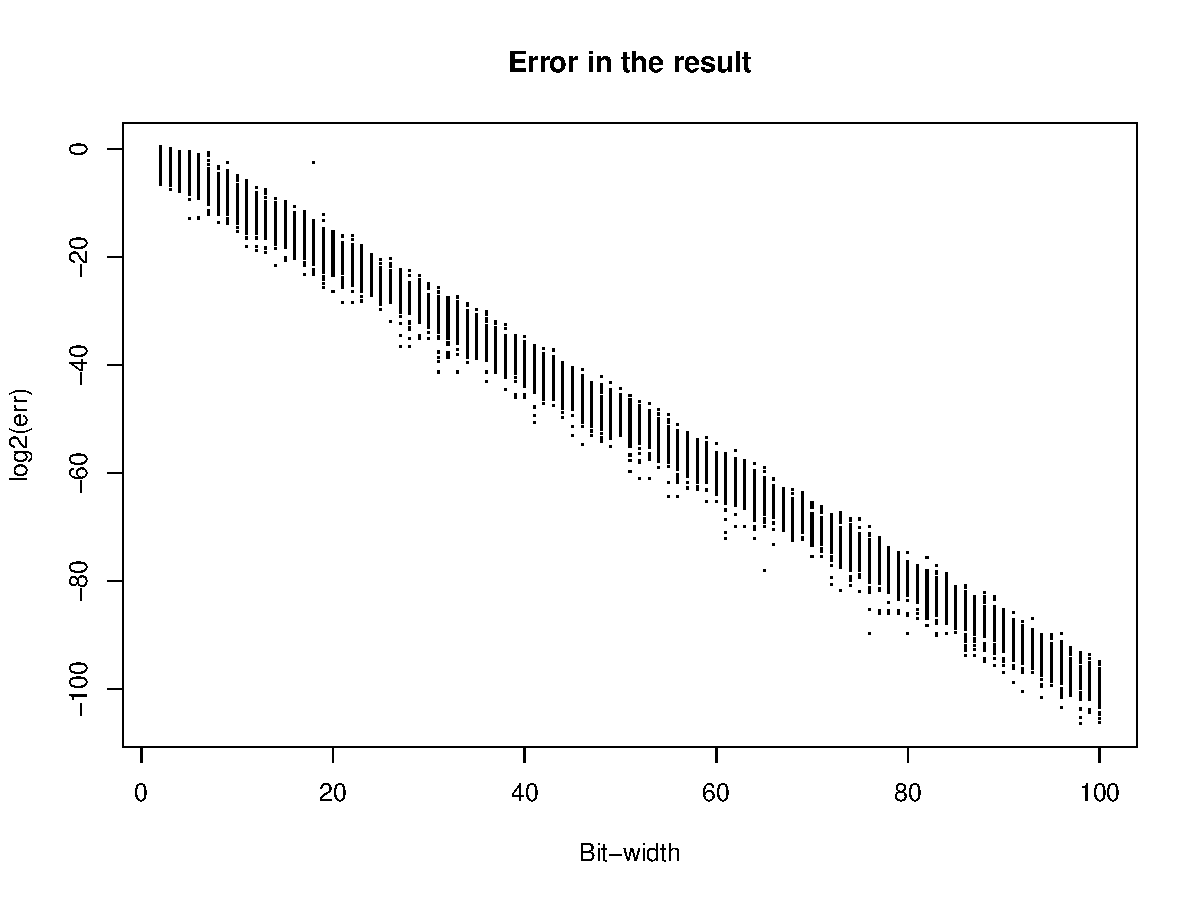
\includegraphics[width=\linewidth]{img/err.pdf}
\end{figure}

\paragraph{Conclusion}
It can be observed that $\log_2 \Delta$ is close to $-b$. More experiments are 
needed to test this hypothesis.

%%%%%%%%%%%%%%%%%%%%%%%%%%%%%%%%%%%%%%%%%%%%%%%%%%%%%%%%%%%%%%%%%%%%%%%%%%%%%%%%
\newpage
\subsection*{Experiment B}

\paragraph{Objective}
Test if the relation between the $\log_2 \Delta$ and $b$ is linear.

\paragraph{Description}
Let $X_b = \log_2 \Delta$ and $Y = b + \overline X_b$. We can now plot $Y$ as 
$b$ grows. If $\overline X_b = -b$, then $Y$ should be 0. For each bit-width $b$ 
in the range $[2, 100]$, a set of 10000 simulations are performed with $n=5$, 
and the sample mean $\overline X_b$ is computed.

\paragraph{Result}
The random variable $Y$ seems to be constant as the bit-width grows, as can be 
seen in the figure~\ref{fig:expB}.
\begin{figure}[h]
	\begin{tikzpicture}
		\begin{axis}[
%			scale only axis,
			xlabel={$b$},
			ylabel={$b + \overline X_b$},
			width=\textwidth,
			height=0.7\textwidth,
			grid = both,
		]
			\addplot+ [
				mark=none,
%				only marks,
%				mark size = 0.5pt
			] table [
				x index = {0},
				y index = {1},
				col sep = space
			] {../data/exp1f.csv};
		\end{axis}
	\end{tikzpicture}
	%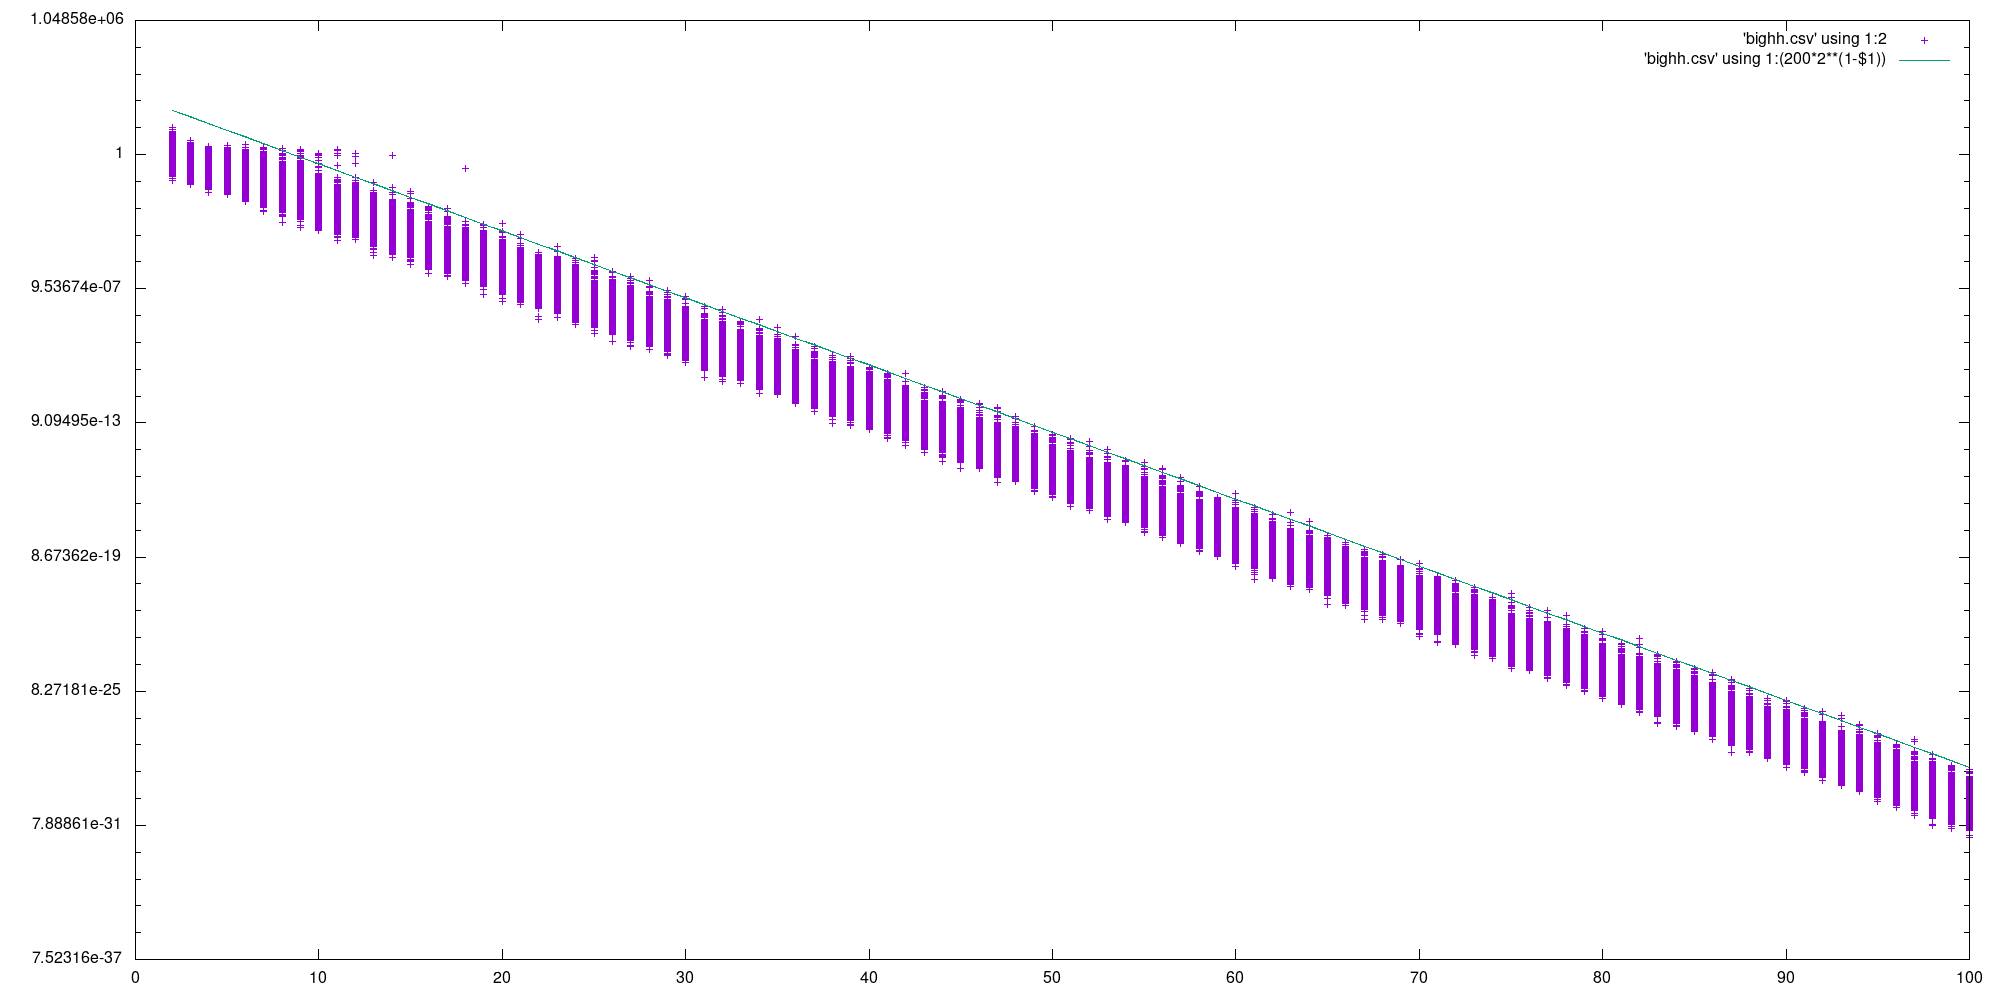
\includegraphics[width=\textwidth]{bighh}
	\caption{Plot of $b + \overline X_b$ as the number of bits $b$ increases.}
	\label{fig:expB}
\end{figure}

\paragraph{Conclusion}
Further statistical analysis reveals that, if the values with $b<5$ are not 
considered, $Y$ is independent of $b$, and has a mean in the interval $2.68691 
\pm 0.00190$ at a confidence level of $0.95$. Then, the relation between 
$\overline X_b$ and $b$ is linear. More experiments are needed to determine if 
the mean of $Y$ is always constant.


%%%%%%%%%%%%%%%%%%%%%%%%%%%%%%%%%%%%%%%%%%%%%%%%%%%%%%%%%%%%%%%%%%%%%%%%%%%%%%%%
\newpage
\subsection*{Experiment C}

\paragraph{Objective}
Test if there is any relation between $Y$ and the precision of each variable of 
the Householder algorithm.

\paragraph{Description}
The precision is now determined by a vector $\V b$, so that each variable used 
in the Householder algorithm is assigned a own $b_i$. Let $\V v$ be the set of
variables. Then $v_1$ is the matrix A, $v_2$ the diagonal, $v_3$ the 
offdiagonal, and the others $v_i$ are the internal parameters of Householder 
algorithm. The variable $v_i$ is set a bit-width of $b_i$. The experiment is 
repeated as in the experiment B, but we only change one $b_i$ at the time, 
selecting a precision from [5,100], while the others are set at 500 bits.

\paragraph{Result}
The experiments show that the variable $v_4$ don't produce any error in the 
output. This variable is a internal scale variable of the Householder algorithm, 
and will be ignored, to show the other variables.

\begin{figure}[h]
	\begin{tikzpicture}
		\begin{axis}[
%			scale only axis,
			xlabel={$b$},
			ylabel={$b+\overline X_b$},
%			ylabel={$\overline Y$},
			width=.85\textwidth,
			grid = both,
%			xmin=0,xmax=100
			legend pos=outer north east,
		]
			\addplot+ table {../data/exp3v0.csv};
			\addplot+ table {../data/exp3v1.csv};
			\addplot+ table {../data/exp3v2.csv};
%			\addplot+ table {../data/exp3v3.csv};
			\addplot+ table {../data/exp3v4.csv};
			\addplot+ table {../data/exp3v5.csv};
			\addplot+ table {../data/exp3v6.csv};
			\addplot+ table {../data/exp3v7.csv};
			\addplot+ table {../data/exp3v8.csv};
			\legend{$v_1$,$v_2$,$v_3$,$v_5$,$v_6$,$v_7$,$v_8$,$v_9$};
		\end{axis}
	\end{tikzpicture}
	%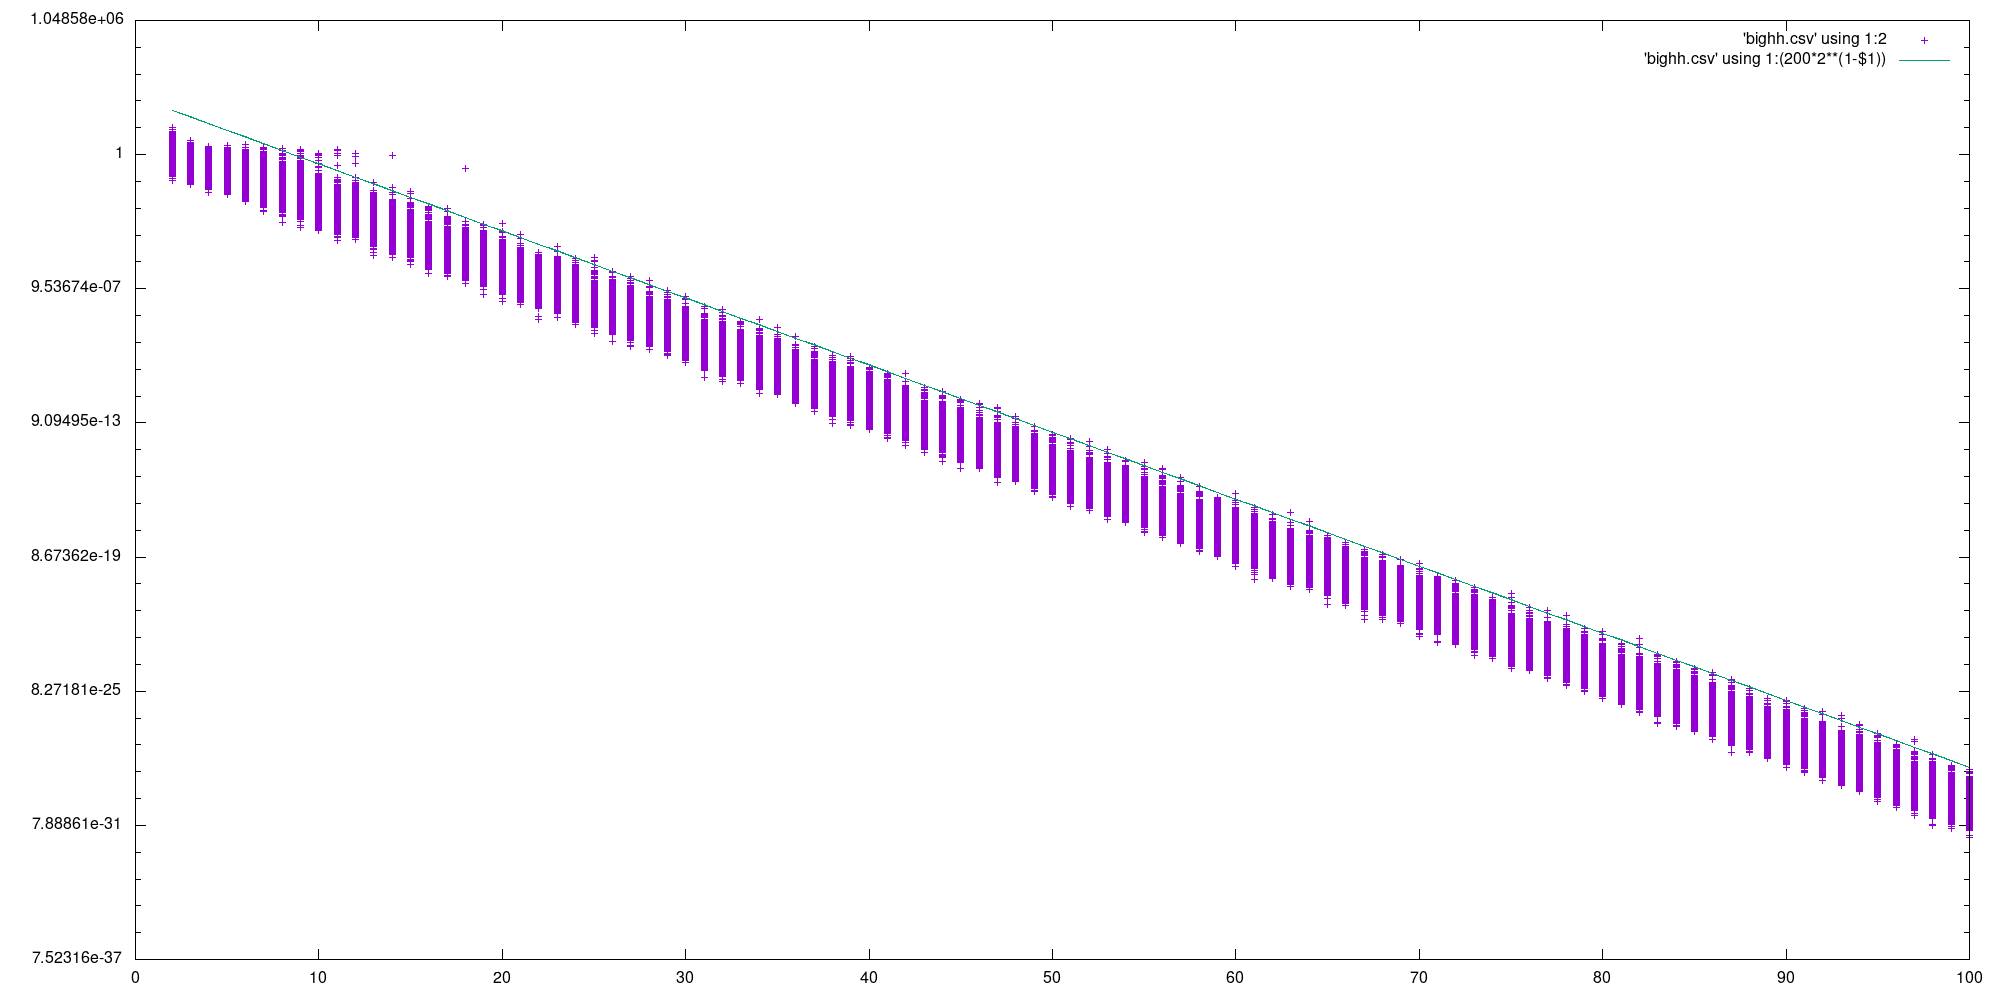
\includegraphics[width=\textwidth]{bighh}
	\caption{Different error mean for each variable.}
	\label{fig:expC}
\end{figure}

\paragraph{Conclusion}
It can be shown that the precision of the variables affect the value of the $Y$, 
and also that is independent of the value of $b$.

%%%%%%%%%%%%%%%%%%%%%%%%%%%%%%%%%%%%%%%%%%%%%%%%%%%%%%%%%%%%%%%%%%%%%%%%%%%%%%%%
\newpage
\subsection*{Experiment D}

\paragraph{Objective}
Test if there is any relation between $Y$ and the condition number $\kappa$ of 
the input matrix.

\paragraph{Description}
The Householder algorithm is executed with a fixed bit-width $b = 50$ and 
compared with the gold result with $b=500$. The error is plotted against the 
logarithmic condition number $\log \kappa$ computed from the input matrix.

\paragraph{Result}
In the figure~\ref{fig:expD} it can be seen that there is no clear relationship 
between the condition number and $Y$.
\begin{figure}[h]
	\begin{tikzpicture}[baseline]
		\begin{axis}[
%			scale only axis,
			xlabel={$\log(\kappa)$},
			ylabel={$b+\log(\epsilon_b)$},
%			ylabel={$\overline Y$},
			width=\textwidth,
			grid = both,
%			xmin=0,xmax=100
		]
			\addplot+ [
				mark=none,
				only marks,
%				mark size = 0.5pt
			] table [
				x index = {1},
				y index = {0},
				col sep = space
			] {../data/exp5b.csv};

		\end{axis}
	\end{tikzpicture}
	%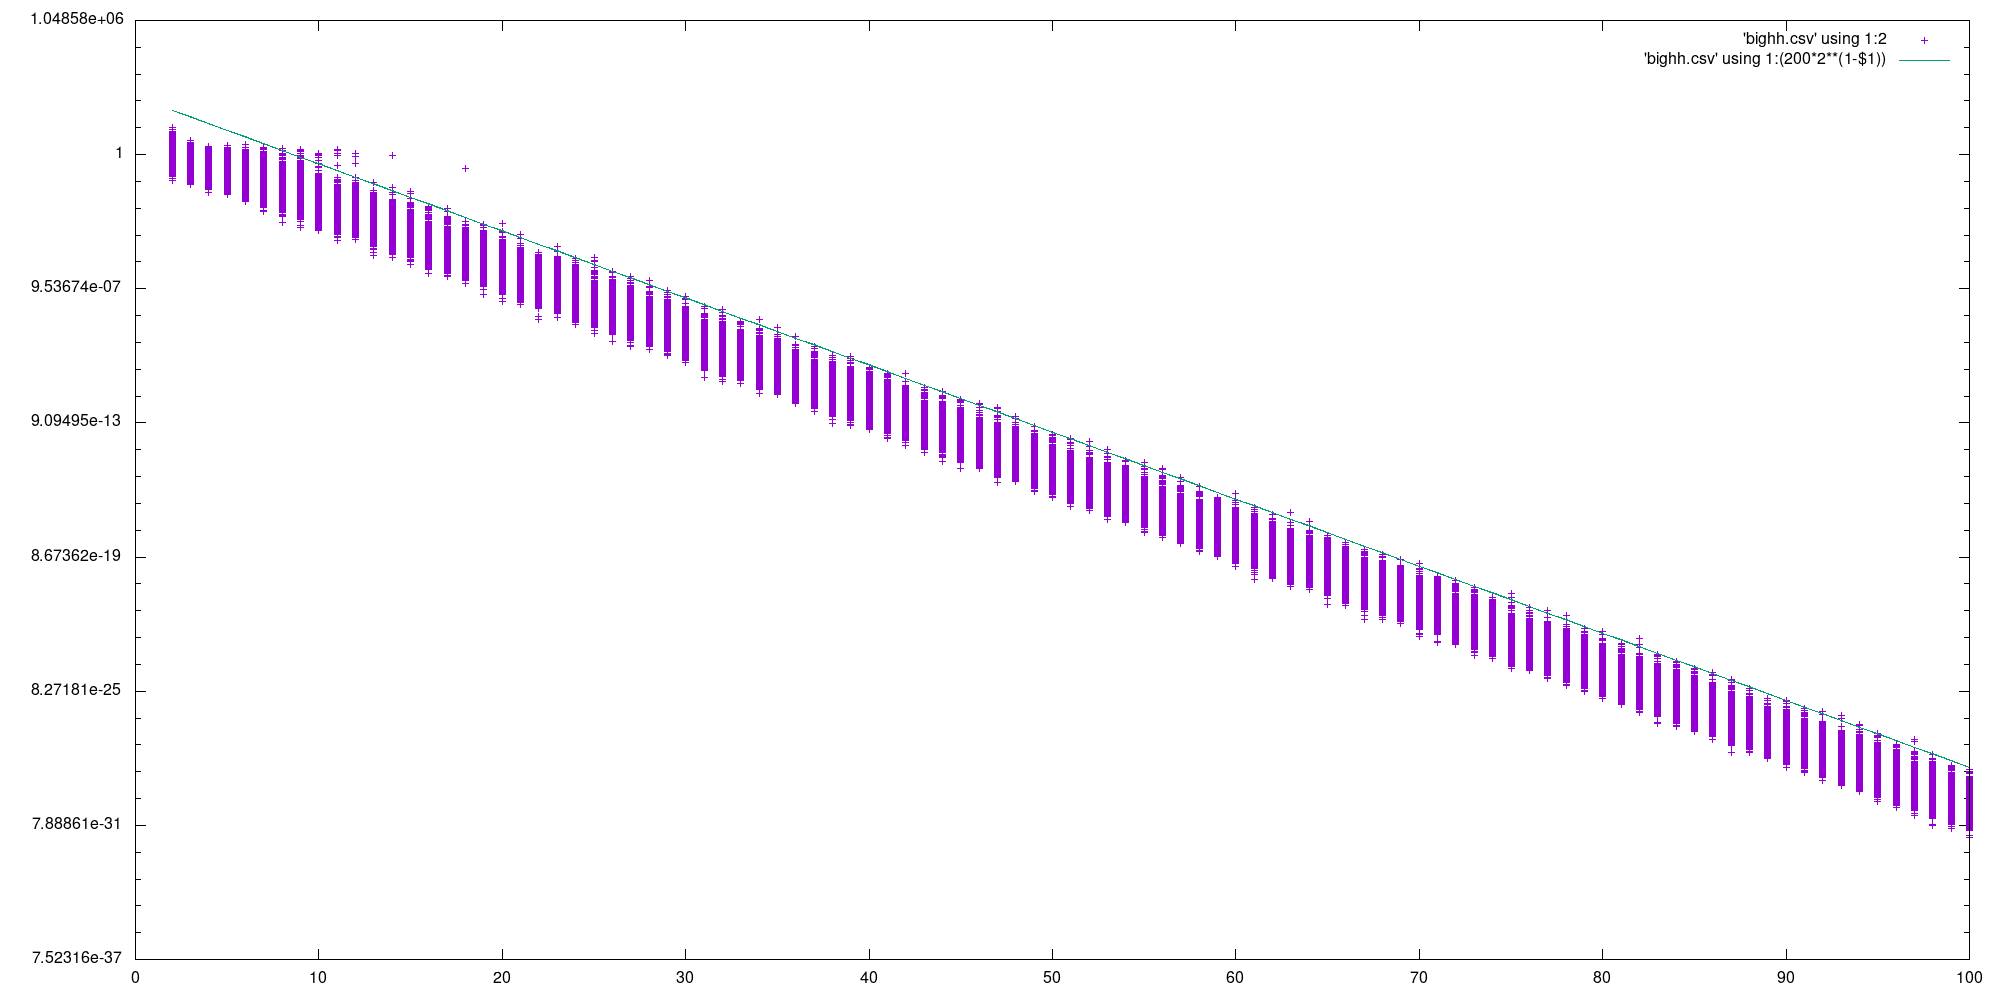
\includegraphics[width=\textwidth]{bighh}
	\caption{Using a fixed bit-width $b=50$ the error is plotted against the 
condition number.}
	\label{fig:expD}
\end{figure}

\paragraph{Conclusion}
The condition number doesn't affect the random variable $Y$ in a meaningful way.

%%%%%%%%%%%%%%%%%%%%%%%%%%%%%%%%%%%%%%%%%%%%%%%%%%%%%%%%%%%%%%%%%%%%%%%%%%%%%%%%
\newpage
\subsection*{Experiment E}

\paragraph{Objective}
Determine the relation between $Y$ and $n$.

\paragraph{Description}
The Householder algorithm is executed varying both the bit-width $b$ and the 
size of the $n \times n$ input matrix. The error is measured by computing the 
norm-2 of the difference between the output vectors of the gold result, and the 
current result.

\paragraph{Result}
The mean of the sample $Y$ is computed from the values with the same input size 
$n$. In the figure~\ref{fig:expE}, the cubic mean $\overline Y^3$ is plotted 
against $n$.


\begin{figure}[h]
	\begin{tikzpicture}[baseline]
		\begin{axis}[
%			scale only axis,
			xlabel={$n$},
			ylabel={$\overline Y^3$},
%			ylabel={$\overline Y$},
			width=\textwidth,
			grid = both,
%			xmin=0,xmax=100
		]
			\addplot+ [
%				mark=none,
%				only marks,
%				mark size = 0.5pt
			] table [
				x index = {0},
				y index = {1},
				col sep = space
			] {../data/exp6d.csv};


		\end{axis}
	\end{tikzpicture}
	\caption{The error $\overline Y^3$ is computed with varying matrix sizes $n$.}
	\label{fig:expE}
\end{figure}


\paragraph{Conclusion}
It can be seen that the relation between $\overline Y^3$ and $n$ seems linear, 
but more data is necessary. A new experiment should be designed to cope with 
bigger matrices.

%%%%%%%%%%%%%%%%%%%%%%%%%%%%%%%%%%%%%%%%%%%%%%%%%%%%%%%%%%%%%%%%%%%%%%%%%%%%%%%%
\newpage
\subsection*{Experiment F}

\paragraph{Objective}
Determine the relation between $Y$ and $n$ when $n$ is big.

\paragraph{Description}
The experiment E is now designed to deal with bigger matrices, and is executed 
with values of $n$ in the range of [500, 5000].  To compute the exact exponent, 
we plot the ratio $Y/\log_2 n$ as $n$ grows.

\paragraph{Result}
It can be seen that the ratio is almost constant, as $n$ grows, and the mean is 
2.78857, represented as a red line in the figure~\ref{fig:expF}.
\begin{figure}[h]
	\begin{tikzpicture}
		\begin{axis}[
%			scale only axis,
			%ymode=log,
			%xmode=log,
			log basis y={2},
			xlabel={$n$},
			ylabel={$Y/\log_2 n$},
%			ylabel={$\overline Y$},
			width=\linewidth,
			height=.7\linewidth,
			grid = both,
%			xmin=0,xmax=100
			legend pos=south east,
			x tick label style={log ticks with fixed point},
		]

			\addplot+ [
%				mark=none,
				only marks,
				mark size = 0.7pt
			] table [
				x index = {0},
				y index = {2},
				col sep = space
			] {../data/exp7a/Y-n3-big.csv};
			\addplot+ [mark=none, red]
				coordinates {(500, 2.78857) (5000, 2.78857)};

		\end{axis}
	\end{tikzpicture}
	\caption{The error $\overline Y$ with varying matrix sizes $n$.}
	\label{fig:expF}
\end{figure}
\paragraph{Conclusion}
The error $Y$ seems to grow with $n$, with a power of $\alpha = 2.78857$,
%
$$Y/\log_2(n) \approx 2.78857 = \alpha $$
%
So, we can compute an approximation of the rounding error $\Delta$ as a function 
of $b$ and $n$, for bigger values of $n$.
%
$$ X = \log_2(\Delta) \approx -b + Y = -b + \alpha \log_2(n) $$
%
And as $\epsilon = 2^{-b}$, we get:
%
$$ \Delta \approx \epsilon \cdot n^\alpha $$


%%%%%%%%%%%%%%%%%%%%%%%%%%%%%%%%%%%%%%%%%%%%%%%%%%%%%%%%%%%%%%%%%%%%%%%%%%%%%%%%
\newpage
\subsection*{Experiment G}

\paragraph{Objective}
Determine if we can use less storage space while maintaining a low error, with 
different precisions in the variables of Householder algorithm, as well as the 
input matrix $A$, and the two vectors diagonal and offdiagonal.  

\paragraph{Description}
In this experiment the variables used in the Householder algorithm are set with 
individual precisions. The input matrix A and the diagonal vectors diagonal and 
offdiagonal are set each with individual precisions.
The golden result is computed using 500 bits of precision in all the variables.  
The storage size is plotted against the error.

\paragraph{Result}
It can be seen in the figure~\ref{fig:expG} the relation between the error and 
the storage size in bits. When the main variables like the input matrix $A$, or 
the diagonal and offdiagonal vectors are assigned a low precision, less space is 
needed, but the error increases. Also, by using a mix of high and low precision 
variables, the error keeps high.

\begin{figure}[h]
	\centering
	\includegraphics[width=.7\textwidth]{img/expG.pdf}
	\caption{The error $\overline Y$ with varying matrix sizes $n$.}
	\label{fig:expG}
\end{figure}

\paragraph{Conclusion}
It seems better to select all precision to the same value, in order to obtain 
the smallest error.


%%%%%%%%%%%%%%%%%%%%%%%%%%%%%%%%%%%%%%%%%%%%%%%%%%%%%%%%%%%%%%%%%%%%%%%%%%%%%%%%
\newpage
\subsection*{Experiment H}

\paragraph{Objective}
Determine the effect of the precision in the different elements in the input 
matrix $A$ and the vector diagonal and offdiagonal, as they change.

\paragraph{Description}
In each step, a random configuration of bits is assigned to each element in the 
matrix and in both vectors. The possible values are $\{8,16,32,64\}$, and are 
selected randomly with a probability of $1/4$ each.

Once the configuration of bits for the data storage is completed, the 
Householder algorithm runs with the internal variables at 64 bits. Then, the 
error is computed from the gold result.

\paragraph{Result}
It can be seen, in red, the configurations now have a big error and use more 
space than the previous experiment.

\begin{figure}[h]
	\centering
	\includegraphics[width=.7\textwidth]{img/expH.pdf}
	\caption{The error $\overline Y$ with varying matrix sizes $n$.}
	\label{fig:expG}
\end{figure}

\paragraph{Conclusion}
Is better to left all the precisions inside the matrix or vectors to the same 
value.



\end{document}
